\chapter{High-voltage electrical system}
\paragraph{} The design and provision of electrical power systems for aerodrome visual and radio navigation aids will be such that an equipment failure will not leave the pilot with inadequate visual and non-visual guidance or misleading information. Therefore, Electrical system will be designed following the regulations from \cite{ICAO2006}, \cite{Sanidad2009} and \cite{Standards2016}.

	\section{Electrical system general design}
	\paragraph{} For the airport electrical system, two independent incoming power sources, coming from widely separated sections of the electricity network beyond the aerodrome, with each supplying separate substations on the aerodrome property will be used. Selection is, therefore, on the basis of least probability of simultaneous failure of both sources. 
	
	Power to the aerodrome main power substation will be supplied at a high voltage (over 110 000 volts). Then the voltage will be reduced on the aerodrome substation (Service Drop stations) to an intermediate voltage (25 000 volts) for distribution within the aerodrome. A further step-down of voltage will be necessary to match the required input voltage of visual aids equipment and terminal solicitations.
	
	Aerodrome reliability will be improved by using a double loop system from independent primary sources operating as open rings fed from two transformers at each station.
	
	The general electric system for the whole airport is detailed on figure \ref{electricScheme}.
	
	\begin{figure}[H]
		\centering
		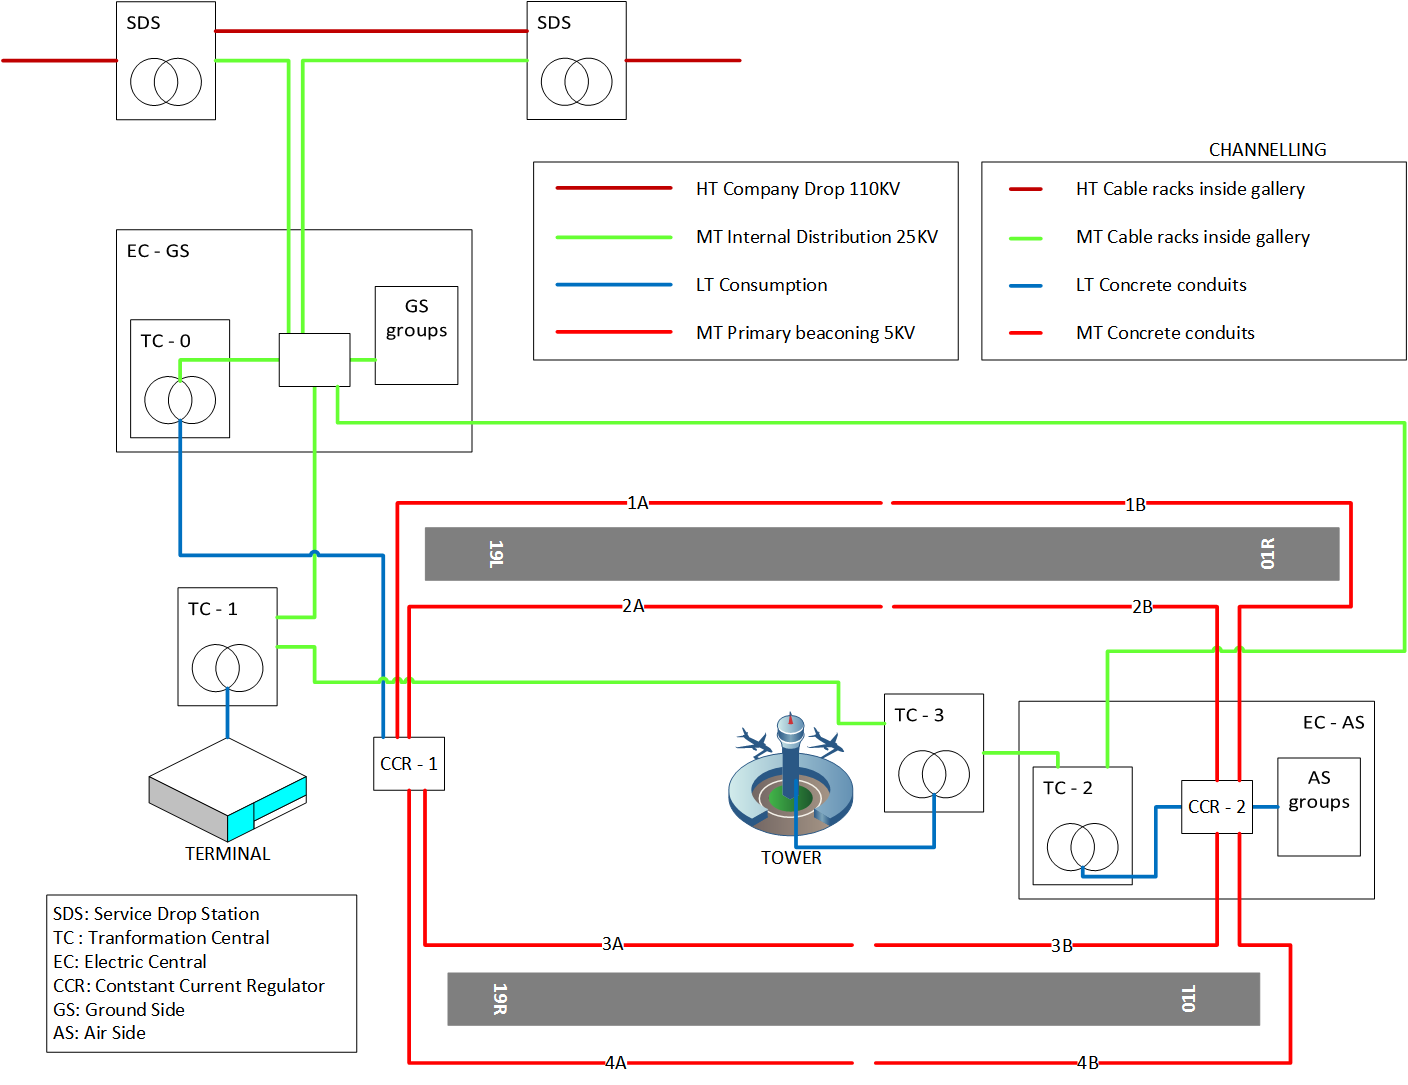
\includegraphics[clip, trim=0cm 0cm 0cm 0cm, width=1.15\textwidth]{./images/electric/esquema_electrico}
		\caption{General electric system scheme}
		\label{electricScheme}
	\end{figure}
	
		
	\section{Connection sub-stations or Service Drop stations}
	\paragraph{} Designated on figure \ref{electricScheme} with SDS (Service Drop Stations), they are located on the top side of the figure. Electricity to the airport will be provided by two different suppliers in order to reduce the chance of the whole system failure.
	
	As previously explained, High Voltage (HV) from the supplier network around 110kV will be drop into the airport network with this connection sub-stations. On figure \ref{substation}, the wiring scheme can be seen: high voltage arrive to the substation making use of the HV towers on the left of the image, then the voltage is steeped-down to an internal distribution voltage level, Medium Voltage 25KV.

	\begin{figure}[H]
		\centering
		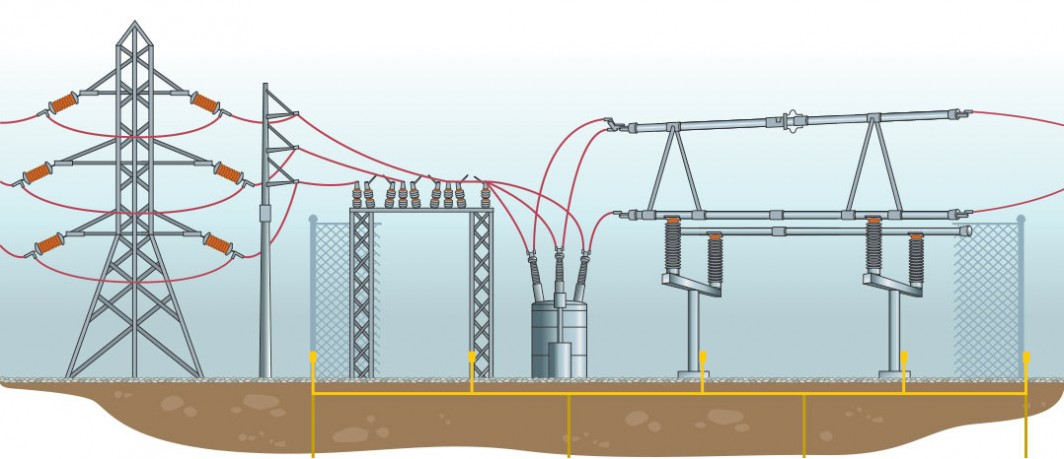
\includegraphics[clip, trim=0cm 0cm 0cm 0cm, width=.8\textwidth]{./images/electric/substation}
		\caption{General electric system scheme}
		\label{substation}
	\end{figure}
	
	\section{Electric power plant}
	\paragraph{} The new airport will have two electric power plants, one for the ground side (EC - GS) and another for the air side (EC - AS). These power plants will work with medium tension values, 25KV. Ground side power plant will be in charge of feeding the terminal building and also the air side power plant. In addition, Air side power plant will supply electricity to all the beaconing circuit, visual aids, tower and aircraft control systems.
	
	Both power plants have an electrical transformation centre to step-down the medium voltage to a Low voltage 380V. Sometimes, as seen on figure \ref{powerplant}, power plants also incorporate a tension regulator centre.
	
	\begin{figure}[H]
		\centering
		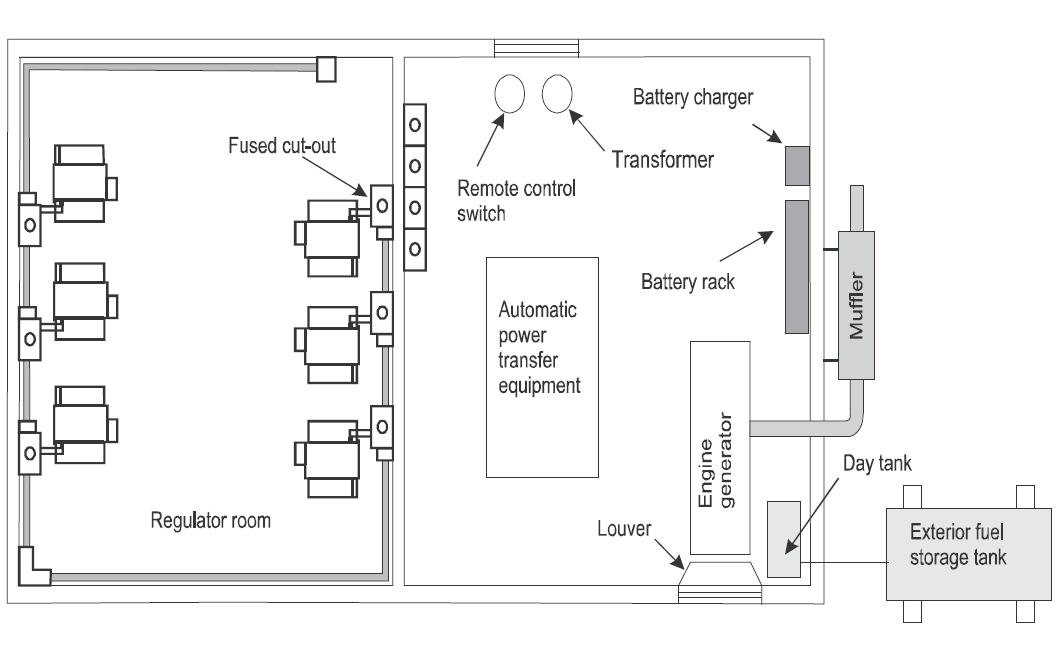
\includegraphics[clip, trim=0cm 0cm 0cm 0cm, width=.7\textwidth]{./images/electric/powerplant}
		\caption{Power plant general scheme.}
		\label{powerplant}
	\end{figure}
	
	In case of the network suppliers electricity failure, power plants, have electricity generator power groups that able to carry on the electricity supply and act as a secondary power supply. 
	
	Air Side power plant, must be able to switch on the secondary power supply in a limited time according to the table \ref{requirements}. Theses circuits requirements will explained in the next sections.  
	
	\begin{figure}[H]
		\centering
		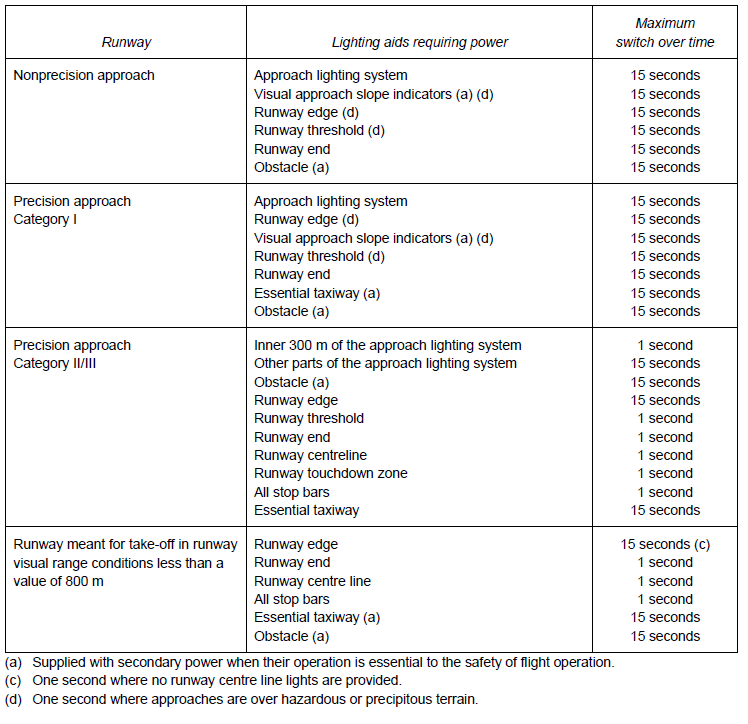
\includegraphics[clip, trim=0cm 0cm 0cm 0cm, width=\textwidth]{./images/electric/requirements}
		\caption{Secondary power supply requirements for visual aids.}
		\label{requirements}
	\end{figure}
	
	\section{Electrical transformation centre}
	\paragraph{} As its name suggest, these devices transform the electricity voltage level. In Bekasi new airport, transformation centres will step-down the medium voltage level 25KV to a Low voltage level for consumption 380V.
	
	Airport will have four transforming centres: two for the beaconing circuits, one for the terminal building and the last one for the tower.
	
	
	\section{Channelling and distribution of the electrical system}
	\paragraph{} Duct-line routes will be selected to balance maximum flexibility with minimum cost and to avoid foundations for future buildings and other structures. Where it may be necessary to run communication lines along with electric power distribution lines, two isolated systems in separate manhole compartments will be provided. Where possible, ducts should be installed in the same concrete envelope.
	
	High Voltage and internal distribution medium tension electric circuit will be transported on metallic cable racks inside underground galleries, accessible by manholes on the surface like figure \ref{manhole}.
	
	\begin{figure}[H]
		\centering
		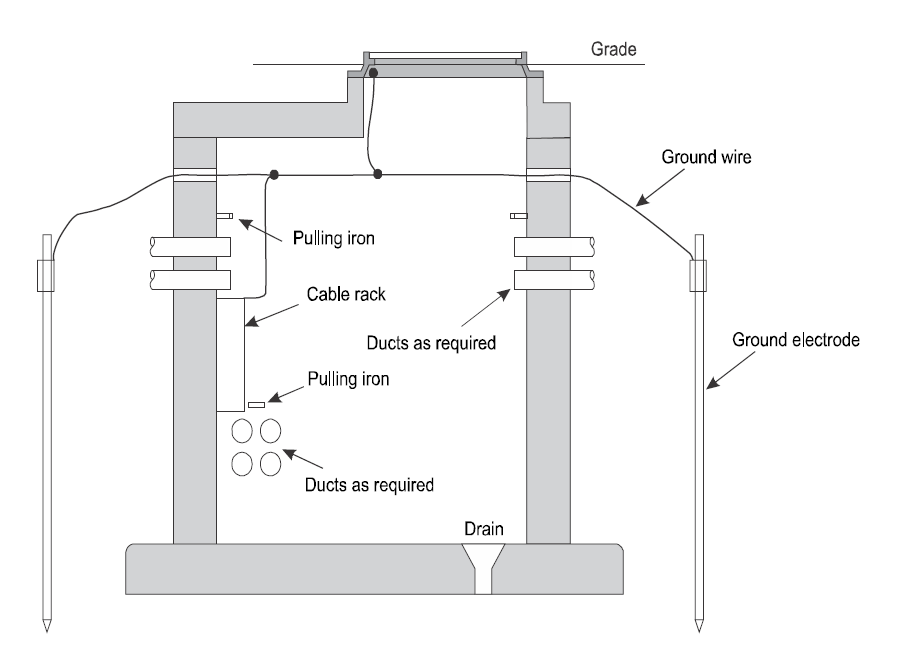
\includegraphics[clip, trim=0cm 0cm 0cm 0cm, width=.8\textwidth]{./images/electric/manhole}
		\caption{General manhole access to gallery distribution.}
		\label{manhole}
	\end{figure}
	
	Note that these galleries will offer the possibility to allocate additional circuits and encased ducts.